\documentclass[twocolumn,10pt]{article}
\usepackage{amssymb}
\usepackage{amsmath}
\usepackage{amsfonts}
\usepackage{array,url,kantlipsum}
\usepackage{lipsum}% http://ctan.org/pkg/lipsum
\usepackage{lineno,hyperref}
\usepackage{graphicx}
\usepackage{float}
\graphicspath{{../Figures/}}
\usepackage[margin=0.75in,tmargin=1in,bmargin=1in]{geometry}
\usepackage{array,multirow}
\usepackage{multirow}
\usepackage{tabu}
\usepackage[table]{xcolor}

\begin{document}
\twocolumn[{%
 \centering
 \LARGE New York City Taxi Data Exploration and Ride Prediction \\[0.5em]
 \large Kurt Nelson \\[1em]
 \normalsize
}]

\section{Project Summary}
Quick taxi pickup times and accurate ride duration predictions ease life in fast-pace cities like New York City (NYC). The project goal is to analyze taxi data collected from two separate carriers in NYC to identify useful patterns for taxi cab drivers, and to develop a prediction model for ride duration. The project is motivated by the Kaggle competition “New York City Taxi Duration.” Time series plots, joint probability mass functions, and heat maps are created and analyzed to learn about spatial and temporal trends in ride frequency, trip duration, and trip length. K-nearest neighbors is also employed on pickup and drop-off locations to investigate spatial connectivity between regions of the city. Finally, ride duration is predicted using gradient boosted trees. The initial training and test root mean squared logarithmic error was 0.4311 and 0.4413, respectively. This project is ongoing. The next stage of the model development is a parameter tuning study on the learning rate, maximum tree depth, and subsample size used to fit the gradient boosted trees. This document serves as project notes and will eventually be expanded into a full report. It is by no means an polished document.

\section{Variables and Data Cleaning}
The competition dataset is based on the 2016 NYC Yellow Cab trip record data made available in Big Query on Google Cloud Platform. The data was originally published by the NYC Taxi and Limousine Commission (TLC), and contains the following fundamental variables:
\begin{itemize}
\item id - a unique identifier for each trip
\item vendor id: a code indicating the provider associated with the trip record
\item pickup datetime: date and time when the meter was engaged
\item dropoff datetime: date and time when the meter was disengaged
\item passenger count: the number of passengers in the vehicle (driver entered value)
\item pickup longitude: the longitude where the meter was engaged
\item pickup latitude: the latitude where the meter was engaged
\item dropoff longitude: the longitude where the meter was disengaged
\item dropoff latitude: the latitude where the meter was disengaged
\item trip duration: duration of the trip in section
\end{itemize}
From the fundamental variables, pickup and drop-off times are broken into month, day of week, and hour using the pandas "todatetime" function. The vincenty distance (method for computing distance between to locations specified by latitude and longitude) between pickup and drop-off locations is then computed using the geopy library. Final trip speed, which is a metric for traffic conditions is computed. 

The data is then cleaned by accepting all data points lying between the bounds defined by the 0.1\% and 99.9\% quantiles for trip duration, distance, and speed. The bounds were selected by plotting marginal probability mass functions and selecting limits that removed unrealistic values. Marginal mass functions are shown in Figure~\ref{fig:MarginalMassFunctions}, and statistics after removal of erroneous data points are shown in Figure~\ref{fig:dataStats}. The small peak on the right tail of the trip duration mass function (middle panel) represents trips to and from JFK airport.

\begin{figure}
\centering
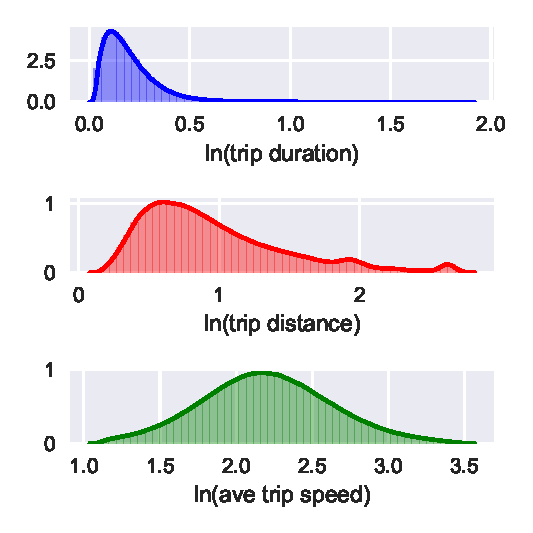
\includegraphics[width=90mm]{marginalMasFunctions}
\caption{Marginal mass functions of the natural logarithm of trip (top panel) durations, (middle panel) distance, (bottom panel) and average speed after removing erroneous data.}
\label{fig:MarginalMassFunctions}
\end{figure}

\begin{figure}
\centering
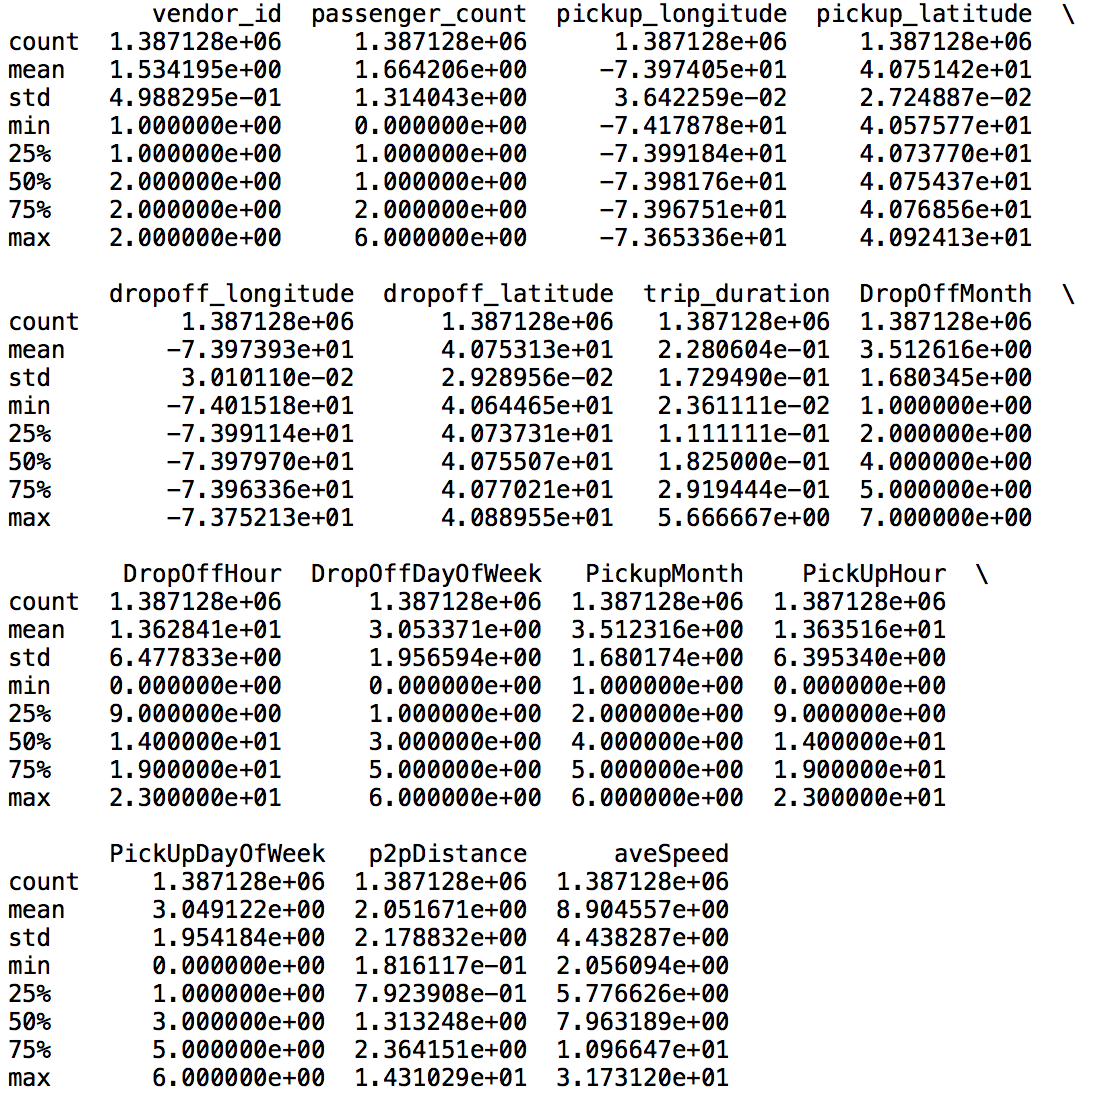
\includegraphics[width=90mm]{dataStats}
\caption{Data set statistics after removing erroneous data. This data should be put in a cleaner format for presentation purposes.}
\label{fig:dataStats}
\end{figure}

\section{K-means Clustering and Spatially Connectivity}
To examine the spatial connectivity of NYC, kmeans-clustering is applied with $k=16$. The number of clusters was selected by plotting pickup and drop-off locations color coded by cluster number, and choosing the $k$-value that partitioned the data in a fashion that aligns with physical intuition of how NYC is geographically divide (Figure~\ref{fig:Clusters}). If a more rigorous approach is desired, something like the "elbow method" can be applied.

\begin{figure}
\centering
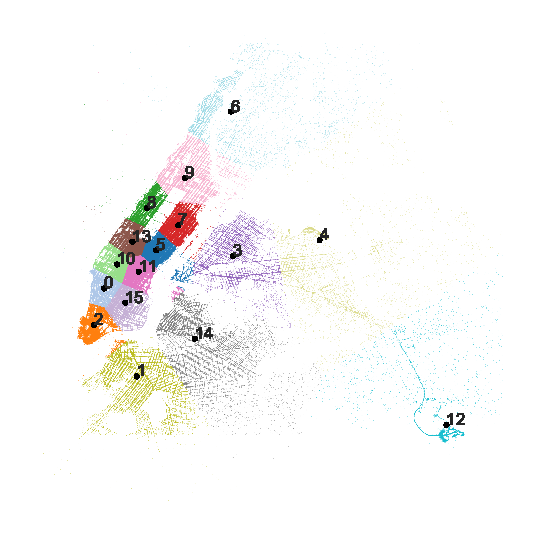
\includegraphics[width=90mm]{kMeansClusters}
\caption{Scatter plot of trip pickup and drop-off locations color coded by cluster number. Black dots show cluster centroids.}
\label{fig:Clusters}
\end{figure}

A joint probability mass function of pickup and drop-off locations is shown in Figure~\ref{fig:JointMassCluster}. The most common ride is a pickup and drop-off in cluster 5 (Upper East Side), which is useful information for taxi cab drivers who prefer short trips. Airport pickups and drop-offs are best for drivers aiming for longer trips. For pickups heading to the airport, drivers should positions themselves in clusters 4 and 11. The most probable pickup location can be computed by row summation of the pickup/drop-off joint probability mass function. This can provide additional information for taxi cab drivers. Additional joint probability mass functions could be created for specific days of the week for further insight. 

Interestingly, commuters commonly travel between clusters 1 (Lower Manhattan) and 5 (Upper East Side). This information is valuable for city planers when deciding regions for increased public transportation.  

\begin{figure}
\centering
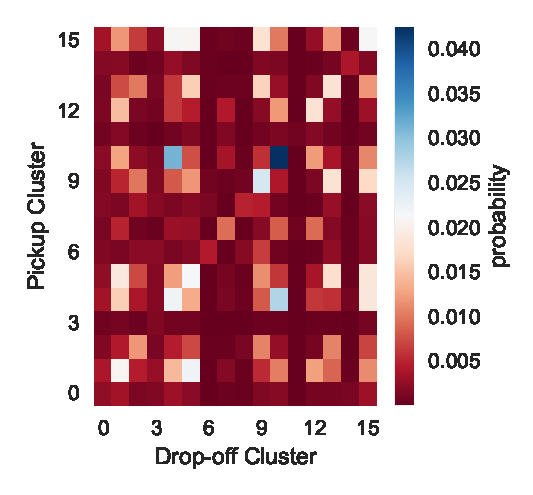
\includegraphics[width=90mm]{JointMassCluster}
\caption{Joint probability mass function .}
\label{fig:JointMassCluster}
\end{figure}

\section{Temporal trends}
Daily-averages of ride duration, distance, and trip speed are shown in Figure~\ref{fig:TimeSeries}. Several notable observations are:
\begin{itemize}
\item Ride duration is inversely correlated to ride distance and speed. People appear to take shorter trips when traffic is bad (slow speed), but the trip duration relatively long.
\item Tuesday through Friday appear to have the worst traffic, shortest rides, and longest trip durations. 
\item People take longer taxi rides on Sunday than any other day. Surprisingly, rides are second longest on Monday. This observation makes me skeptical of the plots (possible shift of days), but it may be explained by more people traveling to and from the airport on Mondays. This prediction can be confirmed from joint probability mass function for pickups and drop-offs on Monday alone.
\item Carrier 2 on average drives shorter distances and has slightly shorter ride durations. This trend might be a reflection of the regions within the city each carrier targets. 
\end{itemize}

\begin{figure}
\centering
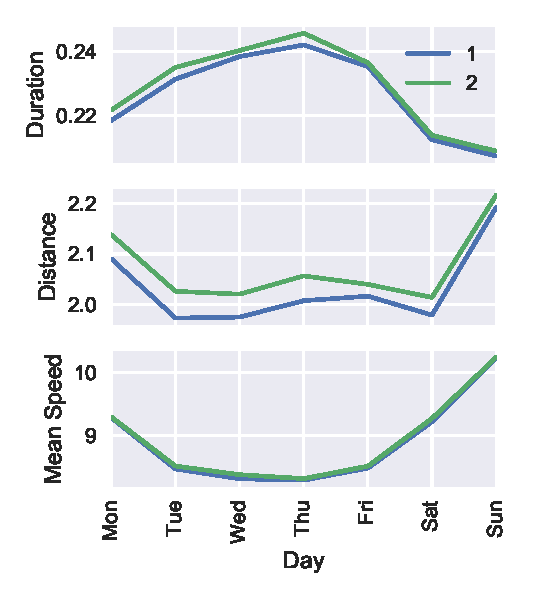
\includegraphics[width=90mm]{TimeSeries}
\caption{Daily-averaged  (top panel) ride duration, (middle panel) distance, and (bottom panel) speed separated by carrier.}
\label{fig:TimeSeries}
\end{figure}

Hourly-averaged heatmaps of trip distance, duration, and speed are shown in Figure~\ref{fig:heatMapDuration}. Several notable observations are:
\begin{itemize}
\item People taking the longest-distance taxi rides tend to do so between 4-5 am on weekdays, and 5-7 am on weekends. However, in general rides are long at night likely because people are returning home after a long work day or night out.
\item The long daily-averaged trip distance for Monday seen in Figure~\ref{fig:TimeSeries} appears to be from night owls spilling into Monday. Trip distances are long between 12-1 am on Monday.
\item From roughly 9 am to 6 pm, traffic is bad (slow speed) during the week. The hourly-averaged speed is fastest from 5-6 am during the week, and 6-7 am on weekends. 
\item Long trip durations are correlated to bad traffic. 
\item Trip duration is again shown to be inversely correlated to trip distance and speed.
\end{itemize}

%\lipsum[1-2]
\begin{figure*}
\centering
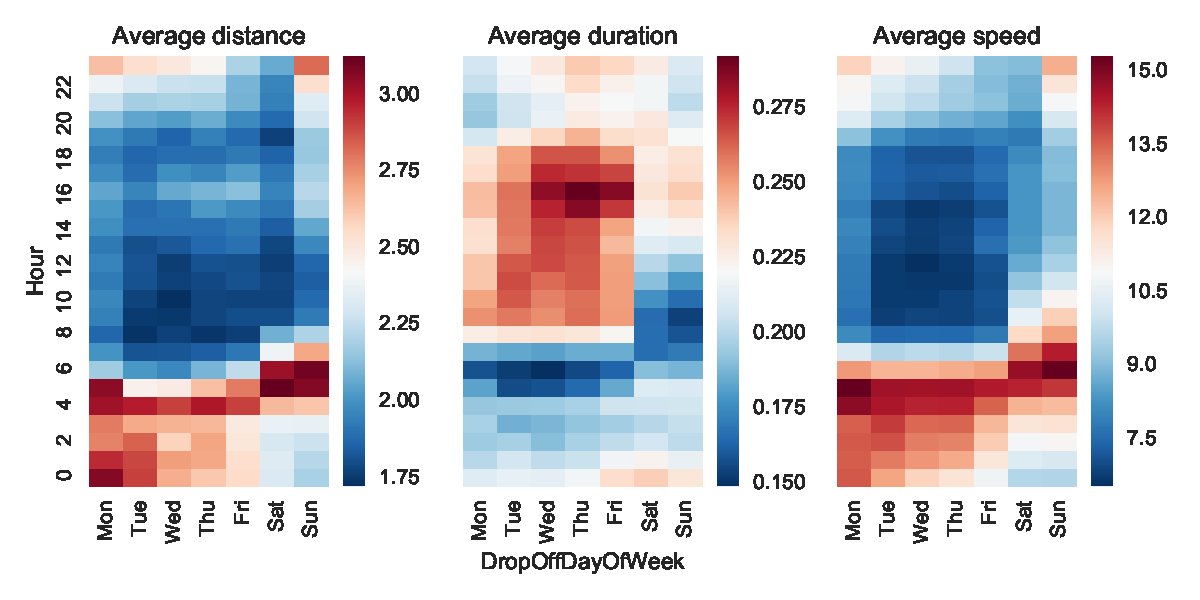
\includegraphics[width=140mm]{heatMapDuration}
\caption{Heatmaps of hourly-averaged trip (top panel) distance, (middle panel) duration, and (bottom panel) speed.}
\label{fig:heatMapDuration}
\end{figure*}
%\lipsum[3-10]

A joint probability mass function based on ride pickup time is shown in Figure~\ref{JointMassFunction}. This plot indicates when taxi services are most used. Several notable observations are:

\begin{itemize}
\item Taxi rides are frequently taken between roughly 5-9 pm during the week, with rides most frequent between 6-7 pm. 
\item There are relatively fewer taxi rides between 12-7 am during the week.
\item During the weekend, people do not frequently take taxis between 4-9 am. The night owls however stay out later on the weekends, with ride frequency increasing between 12-3 pm. NYC is a late night city!   
\item Between roughly 5 pm and 12 am, taxi ride frequently goes up for Monday through Saturday.
\end{itemize}

\begin{figure}
\centering
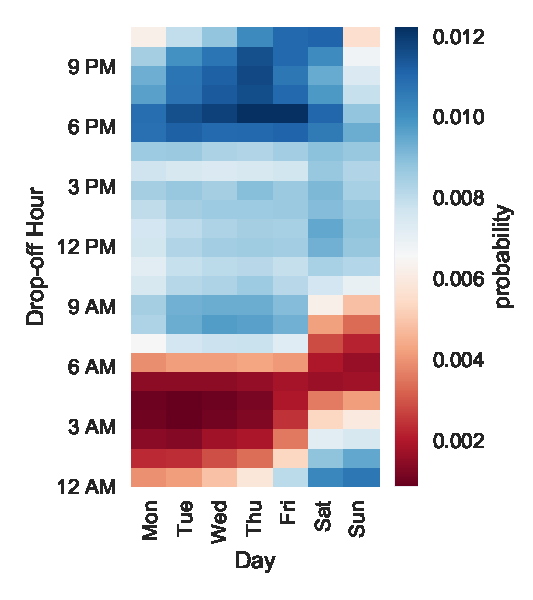
\includegraphics[width=90mm]{JointMassFunction}
\caption{Joint probability mass function based on ride pickup times.}
\label{fig:JointMassFunction}
\end{figure}

The number of pickups and drop-offs for each cluster are plotted as a function of hour of day (Figure~\ref{fig:ClusterCountHour}) and day of week (Figure~\ref{fig:ClusterCountDaily}). These plots should be recreated with legends indicating line labels. More observations will be noted once legends are created, however three quick comments:

\begin{itemize}
\item Generally, ride counts based on hour of day are correlated between clusters.
\item From 6 pm to 5 am, the number of rides for all clusters monotonically decreases.
\item Between approximately 5-8 am, the number of rides at all locations increase.  
\item Additional information on spatial and temporal correlations will be inferred once labels are created. Autocorrelation coefficients can also be computed to enhance the discussion.  
\end{itemize} 

\begin{figure}
\centering
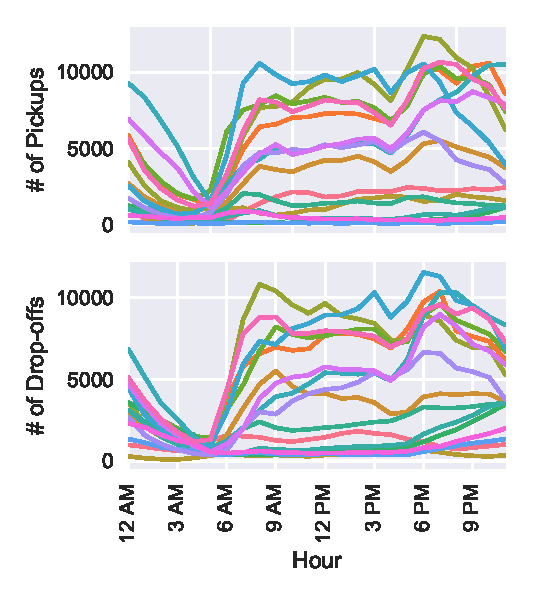
\includegraphics[width=90mm]{ClusterCountHour}
\caption{Number of rides as a function of hour of day for each cluster based on (top) pickup and (bottom) drop-off location.}
\label{fig:ClusterCountHour}
\end{figure}

\begin{figure}
\centering
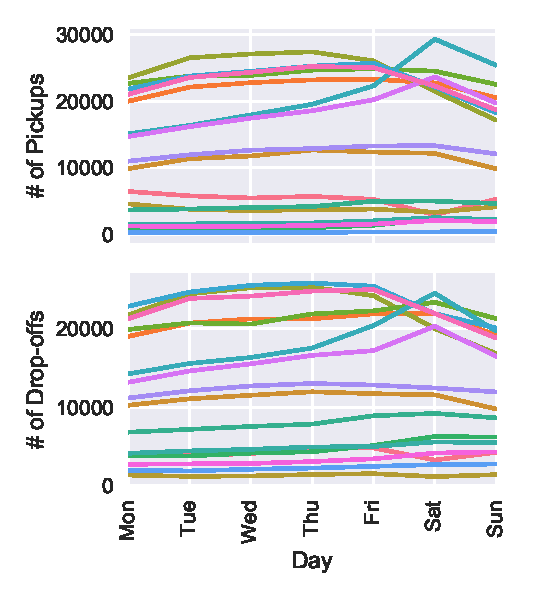
\includegraphics[width=90mm]{ClusterCountDaily}
\caption{Number of rides as a function of hour of day for each cluster based on (top) pickup and (bottom) drop-off location.}
\label{fig:ClusterCountDaily}
\end{figure}
\section{Gradient-boosted Tree}
Notes coming soon!
\end{document}